\chapter{Resultados e Discussão}

\section{Introdução} 

Neste capítulo, será abordado a sequência de testes realizados para o treinamento da RNC, assim como os resultados obtidos. Além disso, será apresentado a eficiência da utilização dos pesos da configuração de treinamento da YOLO que obteve a melhor performance. 

\section{Avaliação do Treinamento} 

Os resultados de desempenho obtidos das RNC, foram estruturados da seguinte forma: realização de uma avaliação do mAP, mAP50, mAP50-95 e recall das versões YOLOv5, YOLOv6 e YOLOv7, com variação do batch de 2 a 16, utilizando o otimizador SGD. Seguido, será avaliado o desempenho da YOLOv8, também com alteração de batch de 2 a 16, e com variação do otimizador. Por fim, será avaliado a performance na identificação de equipamentos, a partir de um conjunto de fotos não treinadas, e avaliar na prática a precisão real de cada configuração dos modelos, aplicadas. 

\subsection{Avaliação do Treinamento} 

Foi discutido na Fundamentação Teórica deste trabalho que a YOLOv8 foi proposta como um modelo superior a suas três últimas versões. Em seu artigo de apresentação, foi comparado a taxa de sucesso da versão 8 contra a versão 5, 6 e 7, quando aplicado a um conjunto de imagens comuns \cite{ultralytics2023yolo}. Por isso, foi realizada a mesma experimentação, a fim de comparar, na configuração padrão de todos hiperparâmetros, se a escolha da oitava versão de fato mostra-se vantajosa. Apenas os parâmetros do batch foram alterados, a fim de verificar o efeito dos lotes no treinamento, conforme também realizado no estudo de \cite{almeida2023batch}.

Por isso, por configuração padrão da rede neural YOLO, entende-se a utilização do otimizador SGD; com a taxa de aprendizado de 0,01; e configuração padrão de entrada das imagens de 640x640. 

\subsection{Resultados e análise do treinamento com a YOLOv5}

Na tabela \ref{tab:yolov5-teste}, apresenta-se o resultado da aplicação da YOLOv5 ao dataset de reatores de núcleo de ar, alterando o valor de batch de 2 a 16.

\begin{table}[!hbt]
    \centering
    \begin{tabular}{|c|c|c|c|c|c|}
    \hline
    \multicolumn{6}{|c|}{\textbf{Otimizador SGD}} \\ \hline
    \textbf{Batch Size} & \textbf{Precisão} & \textbf{Recall} & \textbf{mAP50} & \textbf{mAP50-95} & \textbf{Tempo} \\ \hline
    2                   & 88.724                & 87.456               & 88.785              & 49.821                 & 48.75h             \\ \hline
    4                   & 89.831                 & 89.707               & 95.044             & 55.908                & 37.67h             \\ \hline
    8                   & 92.416                 & 91.922               & 96.197              & 60.488                 & 33.46h             \\ \hline
    16                  & 93.340                 & 90.977               & 95.474              & 56.739                 & 29.53h             \\ \hline
    \end{tabular}
    \caption{Resultados de diferentes tamanhos de batch aplicando YOLOv5}
    \label{tab:yolov5-teste}
\end{table}

\begin{figure}[!h]
    \centering
    \begin{minipage}{1\linewidth}
    \centering
    \captionsetup{justification=centering,margin=0.5cm,font=small}
    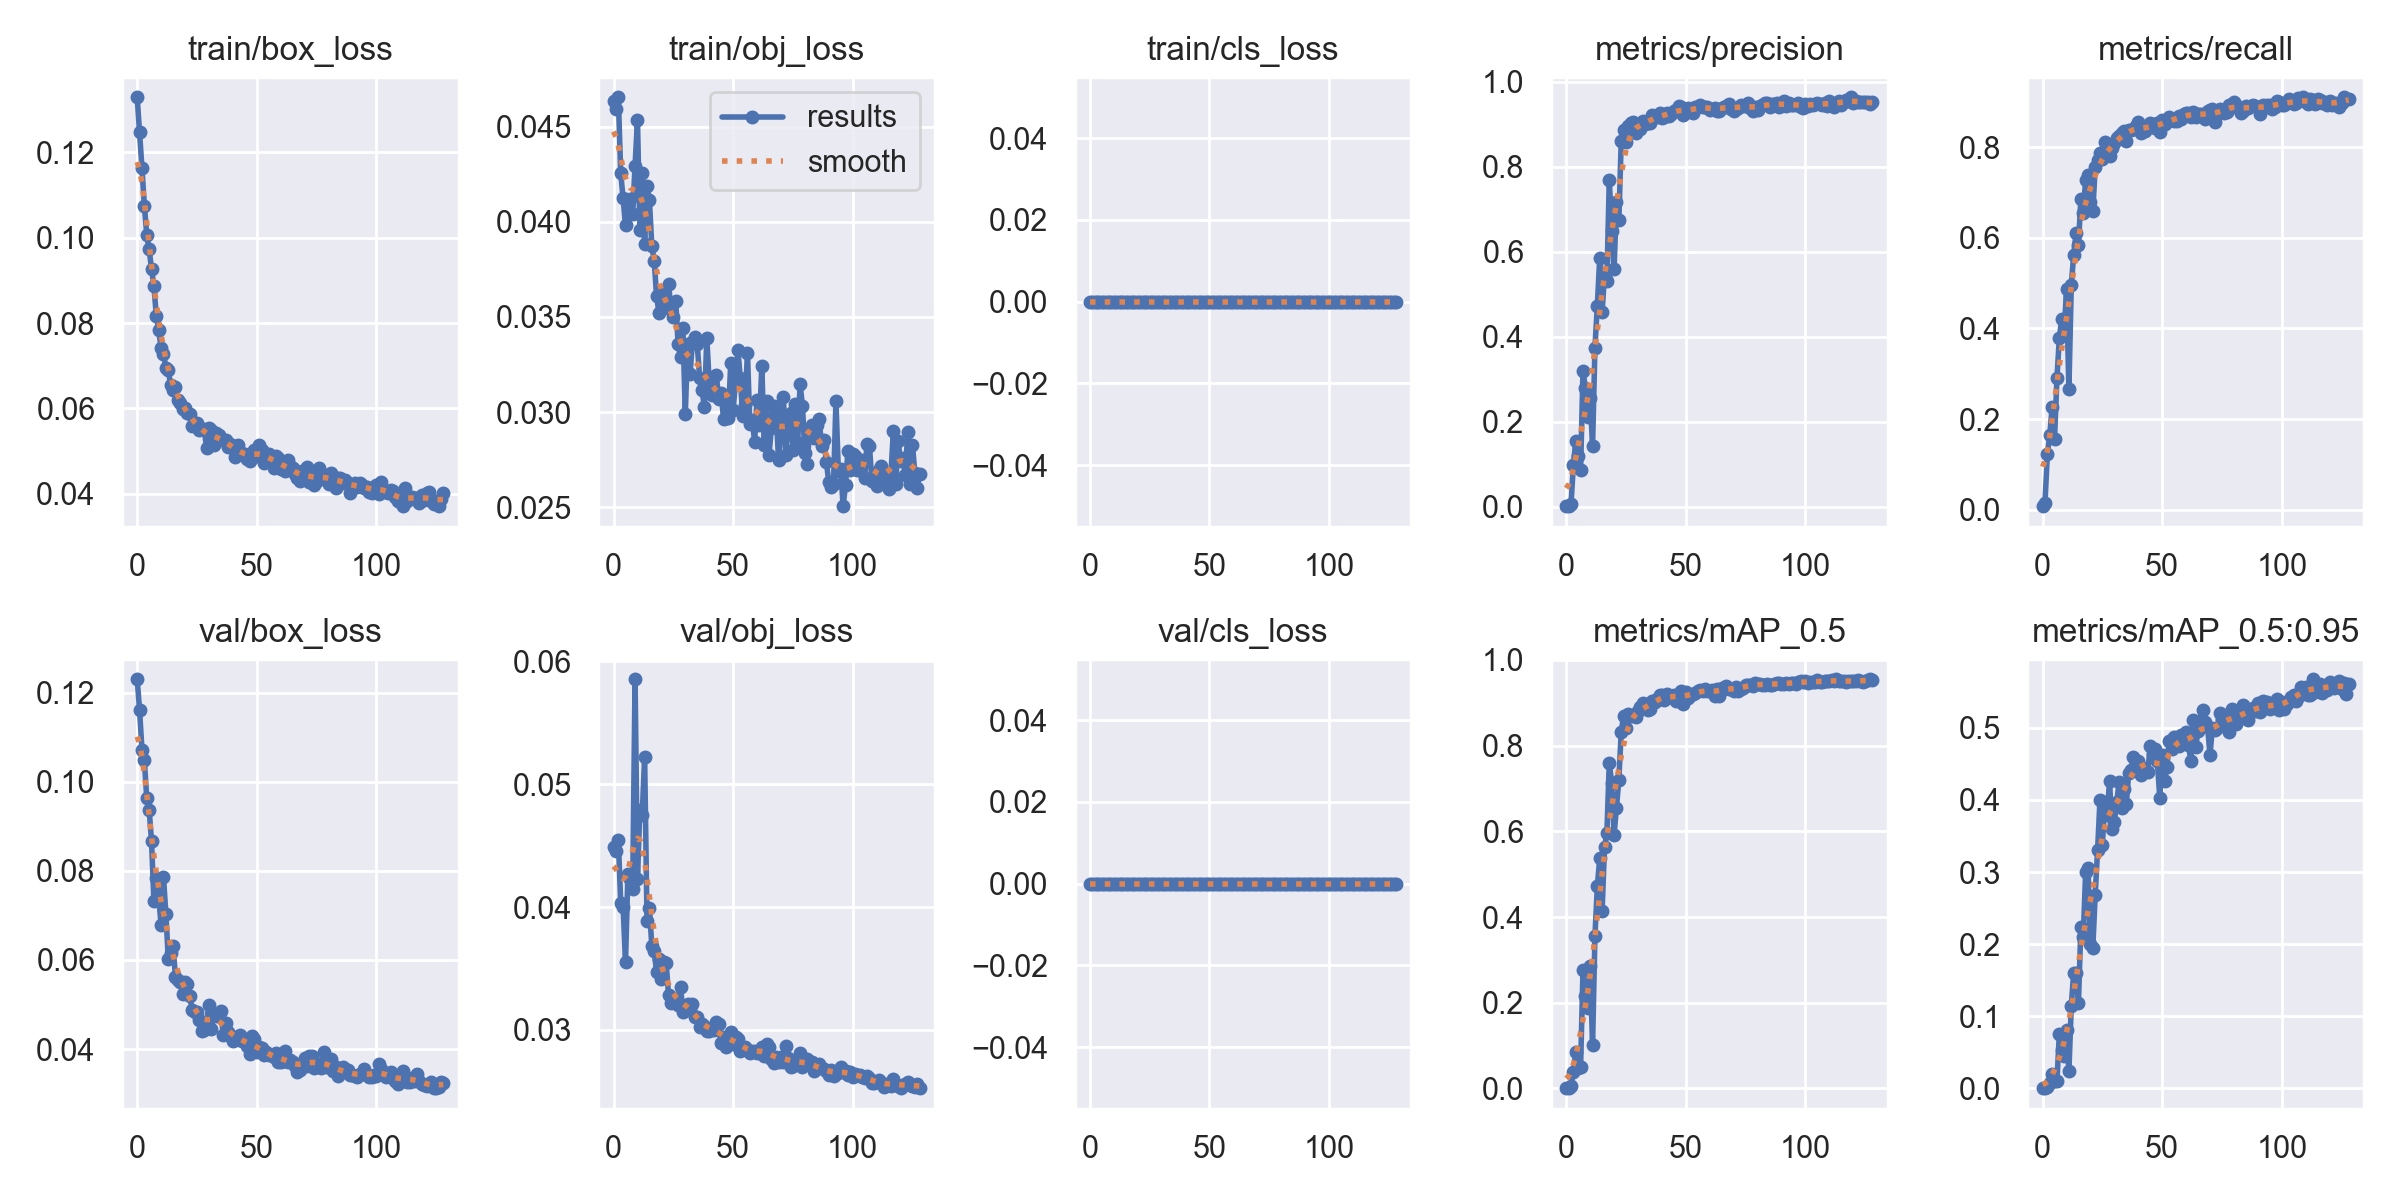
\includegraphics[width=1\linewidth]{img/cap6/results-yolov5-batch-16.png}
    \caption{Gráficos gerados a partir do treinamento com a YOLOv5, utilizando \textit{batch} igual a 16. Nota-se a evolução repentina para uma precisão acima de 90\%}.
    \label{fig:yolov5batch16}
    \end{minipage}
\end{figure}


\subsection{Resultados e análise do treinamento com a YOLOv6}

\begin{table}[!hbt]
    \centering
    \begin{tabular}{|c|c|c|c|c|c|}
    \hline
    \multicolumn{6}{|c|}{\textbf{Otimizador SGD}} \\ \hline
    \textbf{Batch Size} & \textbf{Precisão} & \textbf{Recall} & \textbf{mAP50} & \textbf{mAP50-95} & \textbf{Tempo} \\ \hline
    2                   & 88.523                & 86.225               & 87.895              & 50.705                 & 50.78h             \\ \hline
    4                   & 87.431                 & 90.505               & 94.124             & 54.108                & 39.85h             \\ \hline
    8                   & 91.578                 & 90.592               & 95.298              & 53.128                 & 32.65h             \\ \hline
    16                  & 92.775                & 92.332               & 94.548             & 56.739                 & 30.54h             \\ \hline
    \end{tabular}
    \caption{Resultados de diferentes tamanhos de batch aplicando YOLOv6}
    \label{tab:yolov6-teste}
\end{table}


\begin{figure}[!h]
    \centering
    \begin{minipage}{1\linewidth}
    \centering
    \captionsetup{justification=centering,margin=0.5cm,font=small}
    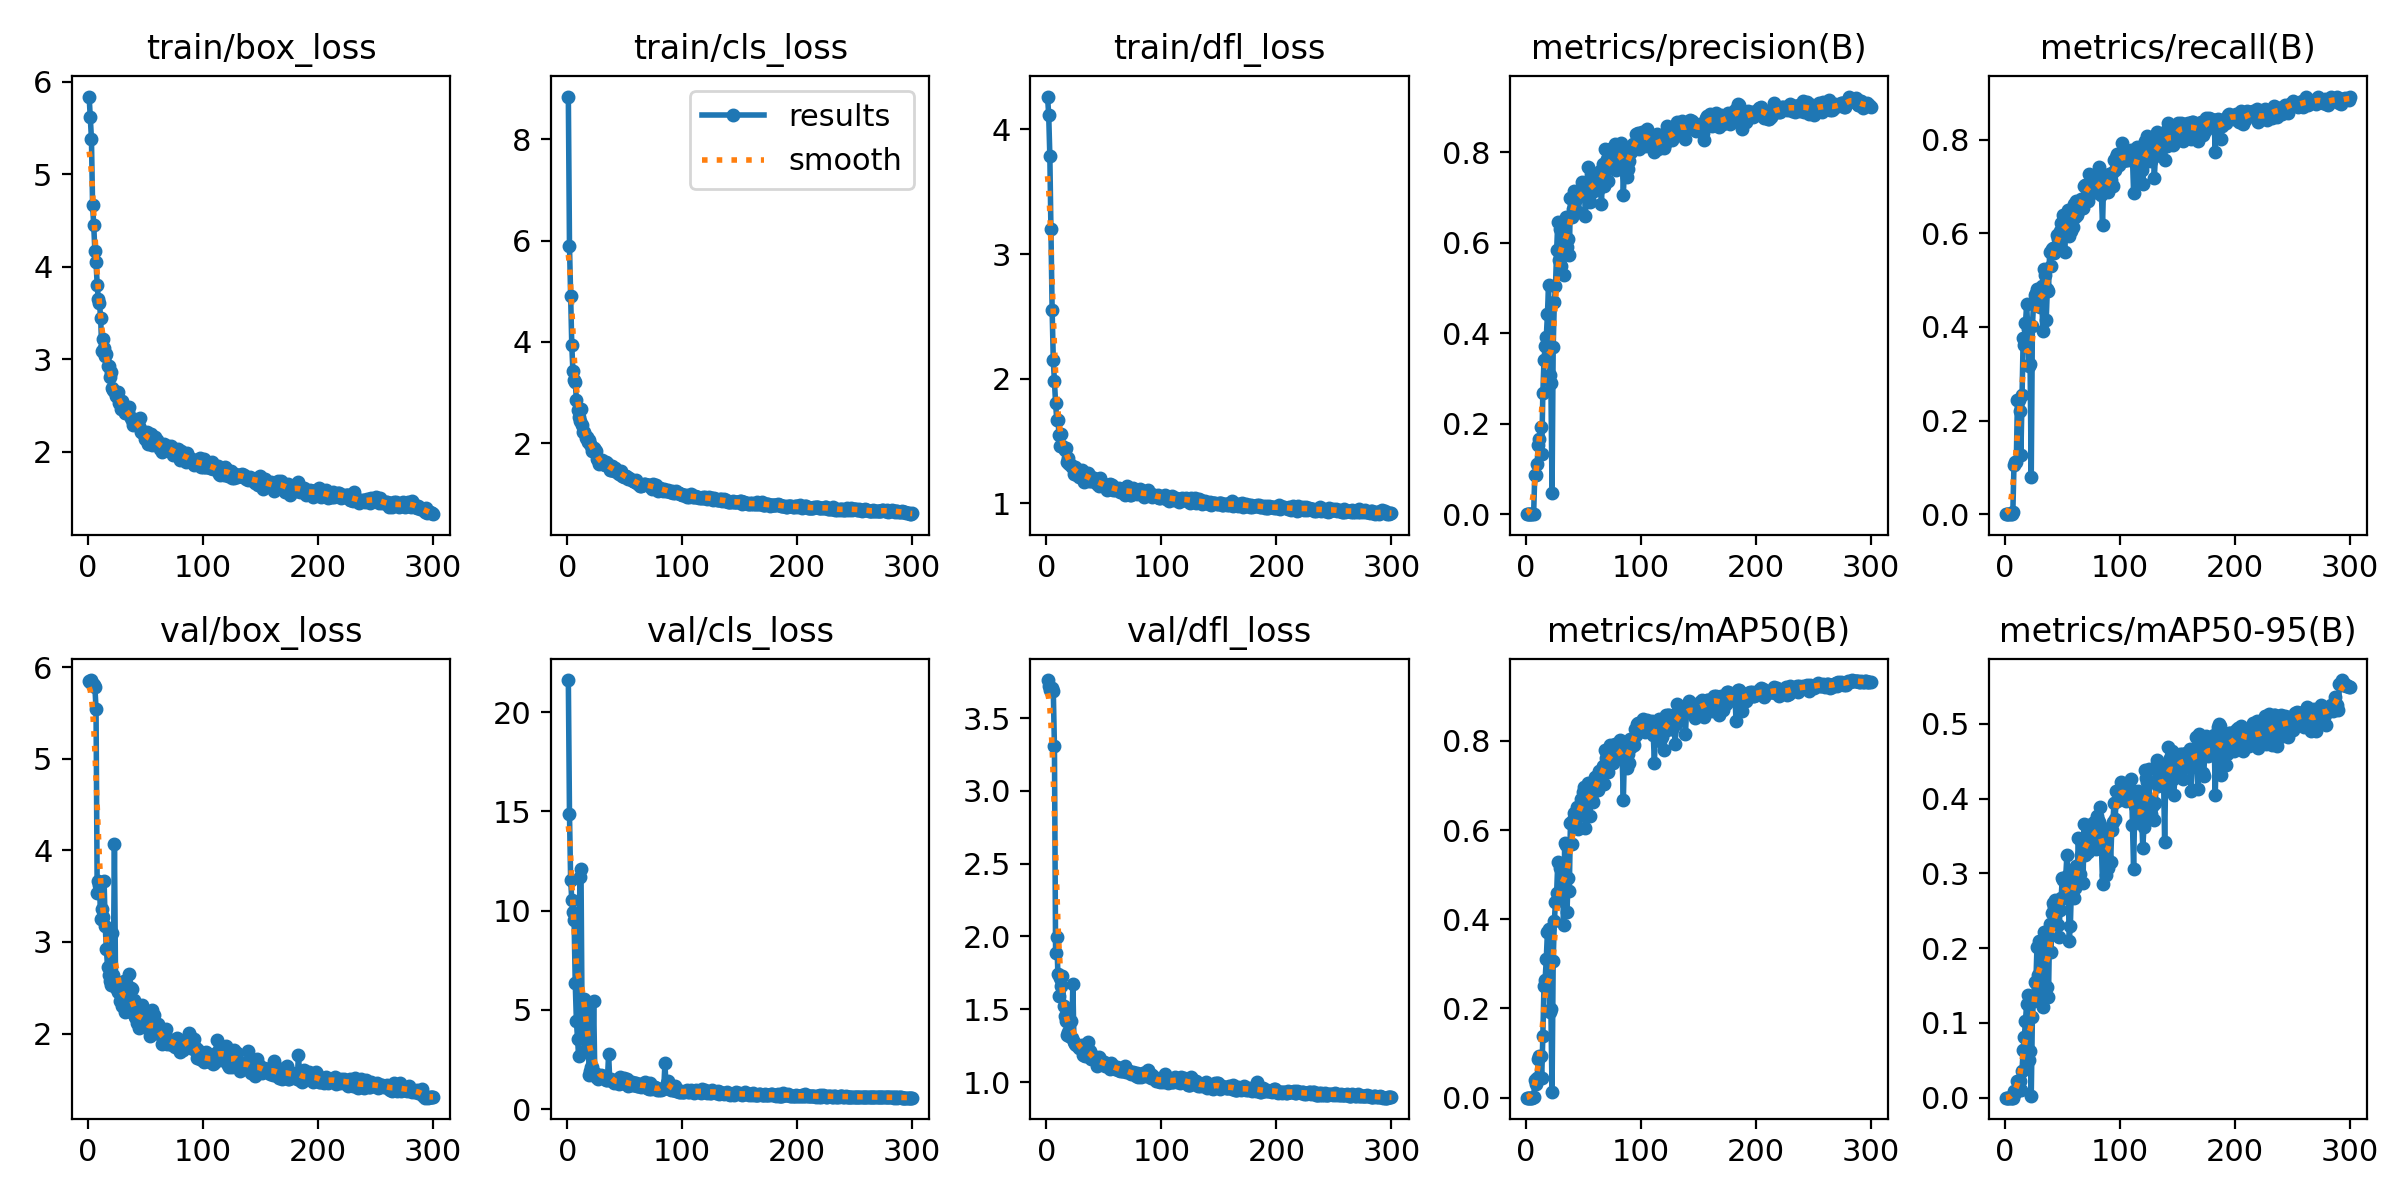
\includegraphics[width=1\linewidth]{img/cap6/results-yolov6-batch-16.png}
    \caption{Gráficos gerados a partir do treinamento com a YOLOv6.}
    \label{fig:yolov6batch16}
    \end{minipage}
\end{figure}


\subsection{Resultados e análise do treinamento com a YOLOv7}

\begin{table}[!hbt]
    \centering
    \begin{tabular}{|c|c|c|c|c|c|}
    \hline
    \multicolumn{6}{|c|}{\textbf{Otimizador SGD}} \\ \hline
    \textbf{Batch Size} & \textbf{Precisão} & \textbf{Recall} & \textbf{mAP50} & \textbf{mAP50-95} & \textbf{Tempo} \\ \hline
    2                   & 66.84                 & 59.45              & 62.42              & 53.45                 & 36.69h             \\ \hline
    4                   & 65.74                & 58.45               & 65.45            & 56.807                & 37.47h             \\ \hline
    8                   & 70.65                 & 59.582               & 68.57             & 54.71               & 38.46h             \\ \hline
    16                  & 73.11                 & 60.882               & 71.35               & 52.53                & 36.14h            \\ \hline
    \end{tabular}
    \caption{Resultados de diferentes tamanhos de batch aplicando YOLOv7}
    \label{tab:yolov7-teste}
\end{table}


O treinamento com a YOLOv7 \ref{tab:yolov7-teste}, apresentou um comportamento diferente das anteriores. Houve graden variação de precisão em pequenos intervalos de tempo...

\begin{figure}[!h]
    \centering
    \begin{minipage}{1\linewidth}
    \centering
    \captionsetup{justification=centering,margin=0.5cm,font=small}
    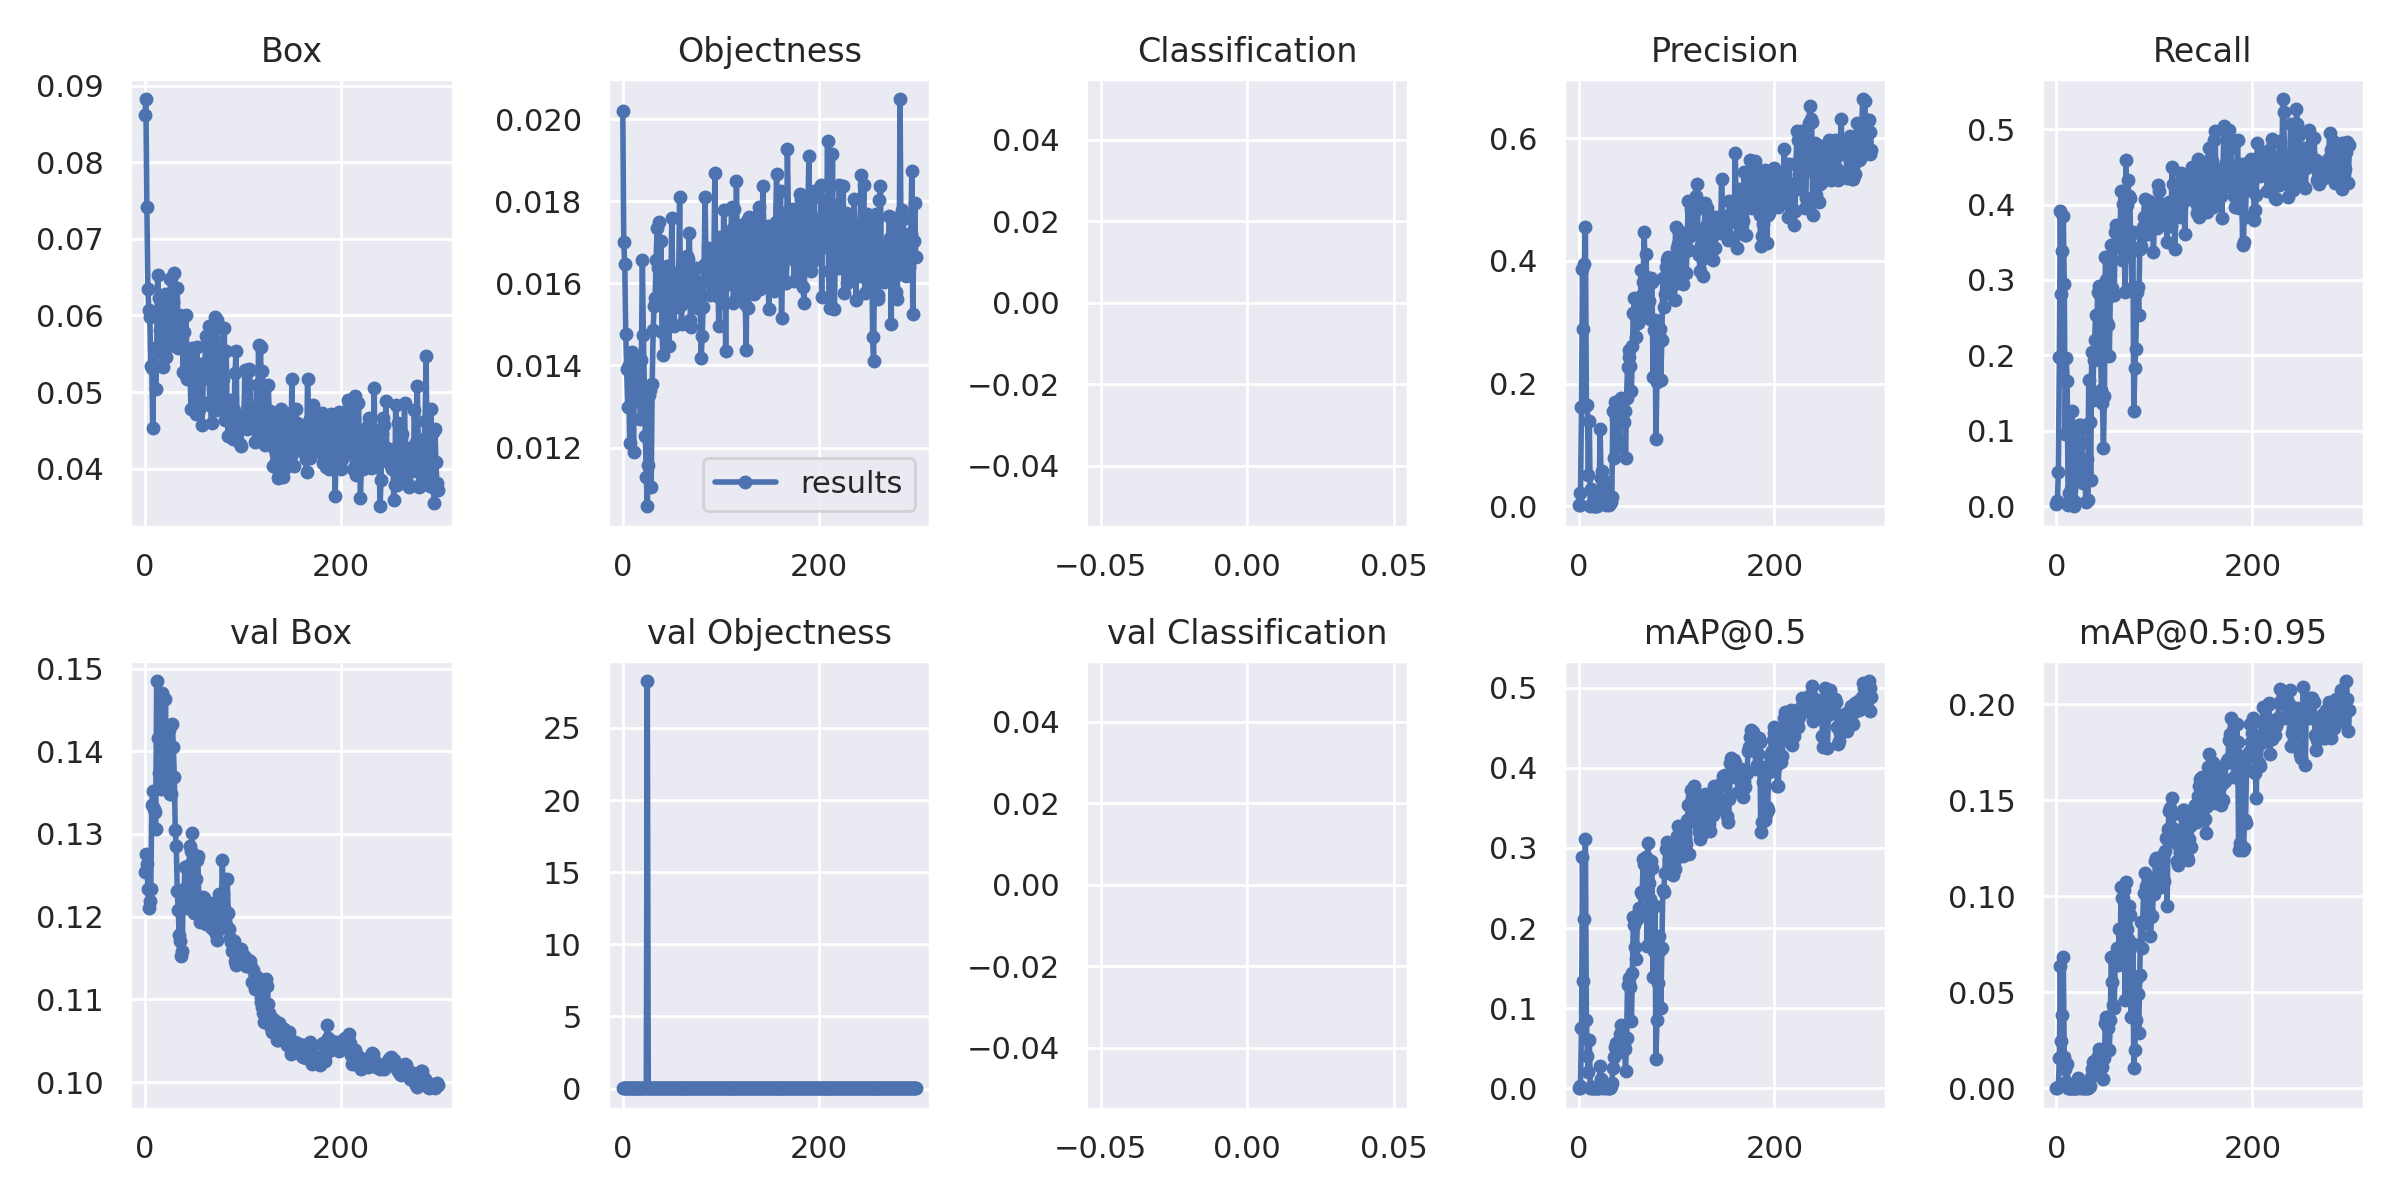
\includegraphics[width=1\linewidth]{img/cap6/results-yolov7-batch-16.png}
    \caption{Gráficos gerados a partir do treinamento com a YOLOv7, utilizando \textit{batch} igual a 16. O comportamento alternato sobressaltou-se nessa arquitetura}.
    \label{fig:yolov5batch16}
    \end{minipage}
\end{figure}

\subsection{Resultados do treinamento com YOLOv8}

\subsection{Análise dos Resultados do Treinamento com YOLOv8}

\begin{table}[!hbt]
    \centering
    \begin{tabular}{|c|c|c|c|c|c|}
    \hline
    \multicolumn{6}{|c|}{\textbf{Otimizador Adam}} \\ \hline
    \textbf{Batch Size} & \textbf{Precisão} & \textbf{Recall} & \textbf{mAP50} & \textbf{mAP50-95} & \textbf{Tempo} \\ \hline
    2                   & 91.323                       & 90.102                     & 94.022                     & 54.987                        & 33.071h                         \\ \hline
    4                   & 92.983                       & 91.857                     & 95.4                       & 57.704                        & 36.548h                         \\ \hline
    8                   & 92.383                       & 91.969                     & 95.006                     & 57.465                        & 31.221h                         \\ \hline
    16                  & 93.654                       & 92.964                     & 96.148                     & 60.269                        & 29.135h                         \\ \hline
    \end{tabular}
    \caption{Resultados de diferentes tamanhos de batch aplicando YOLOv8 e otimizador Adam}
    \label{tab:yolov8-adm}
\end{table}

A Tabela \ref{tab:yolov8-admw} mostra os resultados com o otimizador AdamW, onde a melhoria na precisão e no recall é ainda mais pronunciada. A precisão cresce de 93.886\% para 95.784\%, e o recall sobe de 91.954\% para 95.379\% com o aumento do tamanho do batch. As métricas de mAP50 e mAP50-95 atingem 97.858\% e 68.393\%, respectivamente, para o maior batch size. Embora o tempo de treinamento com AdamW seja consistente, o batch size de 16 proporciona o tempo mais reduzido de 28.013 horas, mostrando uma vantagem competitiva em relação ao Adam.

\begin{table}[!hbt]
    \centering
    \begin{tabular}{|c|c|c|c|c|c|}
    \hline
    \multicolumn{6}{|c|}{\textbf{Otimizador AdamW}} \\ \hline
    \textbf{Batch Size} & \textbf{Precisão} & \textbf{Recall} & \textbf{mAP50} & \textbf{mAP50-95} & \textbf{Tempo} \\ \hline
    2                   & 93.886            & 91.954          & 95.541         & 58.209            & 33.114h        \\ \hline
    4                   & 93.701            & 92.102          & 95.426         & 57.508            & 32.744h        \\ \hline
    8                   & 93.364            & 92.215          & 95.383         & 57.666            & 29.209h        \\ \hline
    16                  & 95.784            & 95.379          & 97.858         & 68.393            & 28.013h        \\ \hline
    \end{tabular}
    \caption{Resultados de diferentes tamanhos de batch aplicando YOLOv8 e otimizador AdamW}
    \label{tab:yolov8-admw}
\end{table}

Por fim, a Tabela \ref{tab:yolov8-sgd} apresenta os resultados com o otimizador SGD, que não só mostra uma melhoria contínua na precisão e no recall, com valores de 96.480\% e 94.718\% para o maior batch size, como também possui os melhores tempos de treinamento. O mAP50 e o mAP50-95 atingem 97.891\% e 68.245\%, respectivamente. O SGD combina o melhor desempenho em termos de métricas com a eficiência de tempo de treinamento, atingindo 27.633 horas para o maior batch size.

\begin{table}[!hbt]
    \centering
    \begin{tabular}{|c|c|c|c|c|c|}
    \hline
    \multicolumn{6}{|c|}{\textbf{Otimizador SGD}} \\ \hline
    \textbf{Batch Size} & \textbf{Precisão} & \textbf{Recall} & \textbf{mAP50} & \textbf{mAP50-95} & \textbf{Tempo} \\ \hline
    2                   & 94.466            & 93.062          & 96.421         & 61.710            & 35.448h        \\ \hline
    4                   & 94.989            & 93.779          & 96.759         & 65.201            & 31.018h        \\ \hline
    8                   & 95.618            & 94.621          & 97.123         & 66.451            & 29.787h        \\ \hline
    16                  & 96.480            & 94.718          & 97.891         & 68.245            & 27.633h        \\ \hline
    \end{tabular}
    \caption{Resultados de diferentes tamanhos de batch aplicando YOLOv8 e otimizador SGD}
    \label{tab:yolov8-sgd}
\end{table}

Em resumo, os dados indicam que aumentar o tamanho do batch geralmente melhora o desempenho do modelo em termos de precisão, recall e métricas de mAP, independentemente do otimizador utilizado. Entre os otimizadores testados, o SGD oferece o melhor equilíbrio entre desempenho e eficiência de tempo, seguido pelo AdamW, que proporciona alta precisão e recall, mas com um tempo de treinamento competitivo. O Adam, embora ainda eficaz, não alcança o mesmo nível de desempenho que os outros dois otimizadores. Esses resultados destacam a importância de escolher cuidadosamente o otimizador e o tamanho do batch para otimizar o treinamento e o desempenho do YOLOv8.

\subsection{Variação de Parâmetros}

Texto da subseção Variação de Parâmetros.






